\section{Evaluation}

\subsection{Microbenchmarks}
\label{q_microbenchmarks}

We evaluate all the queue implementations on a set of microbenchmarks to determine their scalability and performance. The controlled nature of these microbenchmarks allows us to compare particular aspects of each algorithm, such as transactional overhead introduced by STO. All experiments are run on a 100GB DRAM machine with two 6-core Intel Xeon X5690 processors clocked at 3.47GHz. Hyperthreading is enabled in each processor, resulting in 24 available logical cores. The machine runs a 64-bit Linux 3.2.0 operating system, and all benchmarks and STO data structures are compiled with \texttt{g++-5.3}. In all graphs, we show the median of 5 consecutive runs with the minimum and maximum performance results represented as error bars.

\subsubsection{Parameters}

\emph{Value Types}. Each queue benchmark uses randomly chosen integers because the benchmarks do not manipulate the push or popped values and the queue algorithms are agnostic to the actual values being placed in the queue.

\emph{Initial Queue Size}. We run our tests with varying numbers of initial entries in the queue. This affects how often the structure becomes empty, which can cause aborts and additional overhead (as described in the algorithms above). It also affects the number of cache lines accessed: a near-empty queue will never require iterating over values contained in more than one cache line.

\emph{Operations per transaction}. We set the number of operations per transaction to 1 (i.e., the transactions are singleton transactions). By keeping a transaction as short as possible, we maximize the impact of any fixed per-transaction overhead. However, we also minimize the performance hit from the additional transactional overhead required to maintain and commit larger read- or write-sets: running multiple-operation transactions requires multiple-item support in read- and write-sets, creates scenarios of read-my-writes, and increases the number of aborts and retries, all of which incur additional overhead. 
Because most highly-concurrent data structures provide guarantees equivalent to those of singleton transactions, we use singleton transactions when comparing transactional and non-transactional data structures.
Note that our data structure implementations can correctly handle multiple-operation transactions: we simply benchmark them with singleton transactions to compare performance.
 %With single operation transactions, we observe an upper bound on the best performance our data structures can achieve.

\subsubsection{Tests}
    \emph{2-Thread Push-Pop Test}. This test has one thread that performs only pushes and another thread that performs only pops (a traditional ``producer-consumer'' model). Unless the queue is empty, the two threads should never be modifying the same part of the data structure and will never conflict, leading to an abort rate that should be near 0. We use this test to measure the speed of push/pops on the queue under low or no contention. We expect that our transactional queues should perform just as well as the highly-concurrent queues, if not better: while highly-concurrent, non-transactional algorithms are optimized for multi-threaded access, our simpler implementation should be just as fast with low contention and low abort rates.

\emph{Multi-Thread Singletons Test}.
    In this test, a thread randomly selects an operation (push or pop) to perform within each transaction. This keeps the queue at approximately the same size as its initial size during the test. We run this test with different initial queue sizes and different numbers of threads, with each thread performing singleton transactions. Altering the number of threads allows us to benchmark performance under variable amounts of contention and increased abort rates. We expect that the T-QueueO and T-QueueP queues will perform significantly worse once the number of threads is increased, and that these naive synchronization algorithms will underperform synchronization algorithms optimized for contentious situations.

\subsection{Results and Discussion}

We proceed in our discussion by first presenting an overview of our results, and then explaining each in more detail by proposing a sequence of five hypotheses, which we test using the benchmarks described above. For each hypothesis, we use our benchmark results to formulate a conclusion that either refutes or supports the hypothesis.
We provide a few figures that highlight our results; full results (including abort rates) can be found in Appendix~\ref{app:queues}. 

\subsubsection{Overview}
Our results demonstrate the following:
\begin{itemize}
    \item Contentious operations perform better when implemented with a pessimistic, rather than optimistic, approach.
    \item Fixed overhead from bookkeeping STO wrapper calls is negligible.
    \item The flat combining technique is a highly effective synchronization technique for queues, and the flat combining, non-transactional queue outperforms all transactional and concurrent queues.
    \item Performance of the transactional flat combining queue underperforms all transactional queues. The performance loss comes from the greater number and greater complexity of flat combining calls that are necessary to convert the non-transactional flat combining queue to a transactional one.
\end{itemize}


\subsubsection{Hypothesis 1: Pessimistic execution outperforms optimistic execution on contentious operations.}
\begin{figure}[H]
    \centering
	\begin{minipage}{0.75\textwidth}
        \boxed{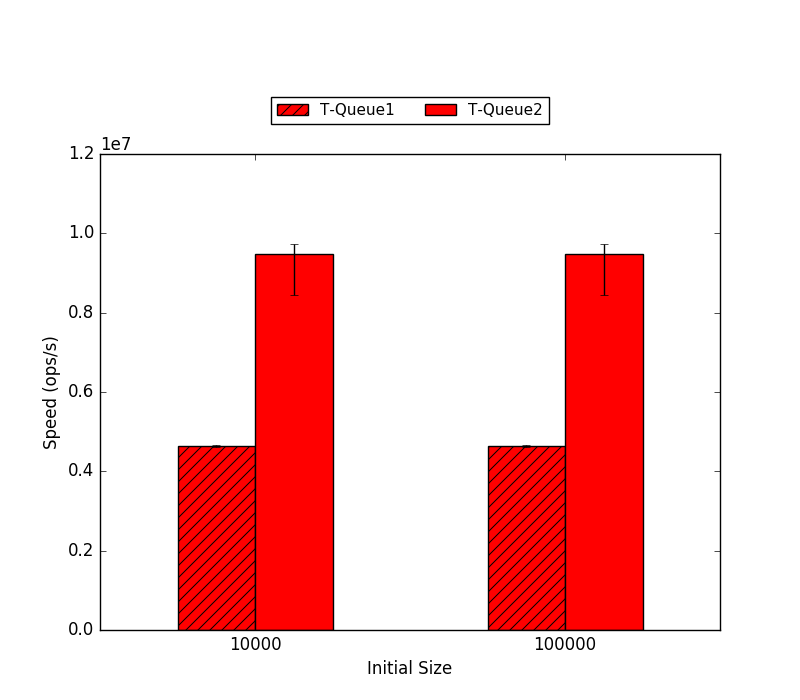
\includegraphics[width=\textwidth]{fcqueues/stoQ:PushPop.png}}
        \caption*{Push-Pop Test (2 threads)}
        \vspace{12pt}
	\end{minipage}
	\begin{minipage}{0.75\textwidth}
        \boxed{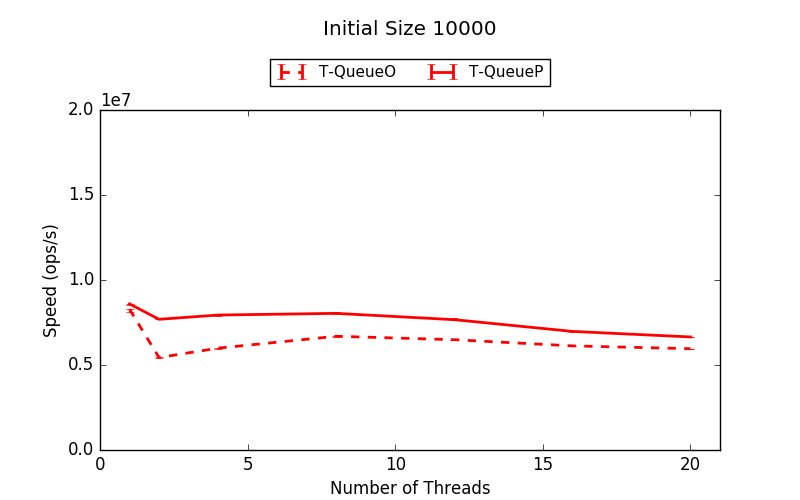
\includegraphics[width=\textwidth]{fcqueues/stoQ:RandSingleOps10000.png}}
        \caption*{Multi-Thread Singletons Test}
	\end{minipage}
    \caption{T-QueueO vs. T-QueueP Performance}
    \label{fig:stoqs}
\end{figure}


We test this hypothesis by comparing the performance of the T-QueueO and T-QueueP queue. These two queues differ only in that a thread running on the T-QueueP queue locks the queue immediately when it performs a transactional pop, therefore pessimistically assuming that any other thread accessing the queue will cause a conflict with its pop operation.

The comparative performance of the T-QueueO and T-QueueP (Figure~\ref{fig:stoqs}) demonstrate the effectiveness of a pessimistic approach to the pop operation. T-QueueP's performance is double that of T-QueueO's performance on the Push-Pop Test, even with triple the abort rate. This likely occurs because the abort rate is still relatively low (at 1.5\%). T-QueueP performs slightly better on the Multi-Thread Singletons Test, likely because of its significantly lower abort rate (1/3 that of the T-QueueO): this result supports that a pessimistic approach to contentious operations such as pop benefits performance. 
%Because of its higher performance, we use T-QueueP as a baseline reference in all future tests.

\vspace{12pt}
\noindent\fbox{\begin{minipage}{\textwidth}
    \textbf{SUPPORTED}: T-QueueP outperforms T-QueueO, indicating that a pessimistic approach is more appropriate for contentious operations.
\end{minipage}}

\begin{figure}[H]
    \centering
	\begin{minipage}{0.75\textwidth}
        \boxed{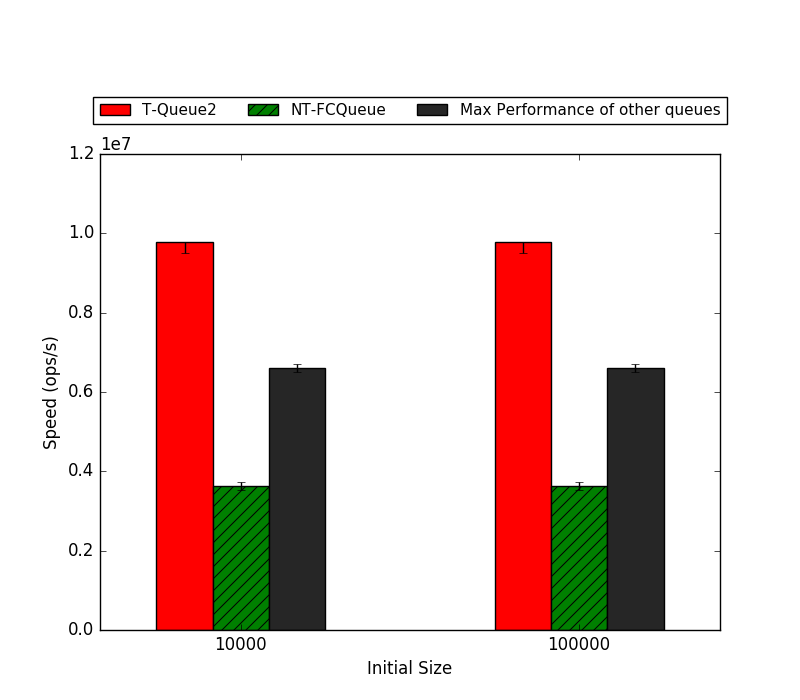
\includegraphics[width=\textwidth]{concurrent/Q:PushPop.png}}
        \caption*{Push-Pop Test (2 threads)}
        \vspace{12pt}
	\end{minipage}
   	\begin{minipage}{0.75\textwidth}
        \boxed{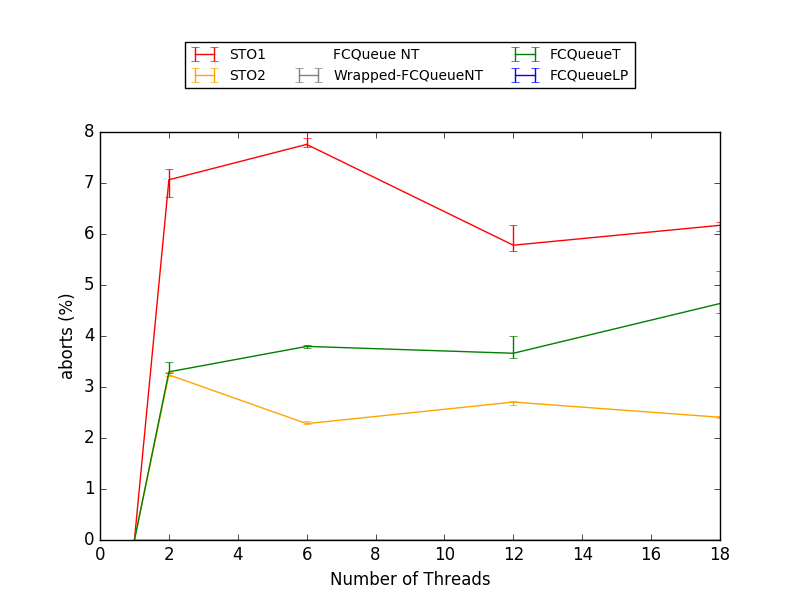
\includegraphics[width=\textwidth]{concurrent/Q:RandSingleOps10000.png}}
        \caption*{Multi-Thread Singletons Test}
	\end{minipage}
        \caption{Non-transactional, concurrent queue performance compared to transactional queue performance}
    \label{fig:ntqs}
\end{figure}

\subsubsection{Hypothesis 2: Under low contention, a transactional queue with a naive concurrent algorithm performs reasonably well compared to the best concurrent, non-transactional queue algorithms.}

We benchmark a set of the best-performing highly-concurrent queue algorithms against our transactional queue implementations, the T-QueueO and T-QueueP, using our low-contention test (the 2-Thread Push-Pop test) that is also optimized for a low abort rate. This acts as a best-case scenario for the T-QueueO and T-QueueP algorithms. Selected results are shown in Figure~\ref{fig:ntqs}.

Our implementation of the non-transactional flat combining queue, which we call NT-FCQueue, uses the flat combining queue implemented by the authors of the flat combining paper~\cite{flatcombining} (with minor modifications to remove memory leaks). Our implementations of the other highly-concurrent queues are taken from the open source Concurrent Data Structures (CDS) library implementations~\cite{libcds}. 

Out of the concurrent, non-transactional queues tested, the Moir queue~\cite{queue2} consistently performs best on the 2-Thread Push-Pop Test; however, we note that performance does not differ significantly between the different concurrent queues besides the NT-FCQueue. The NT-FCQueue appears to perform particularly poorly with low numbers of threads. Most importantly, the T-QueueP outperforms all queues by at least 150\% on the 2-thread Push-Pop test. This test incurs the least contention and transactional overhead to track simply how fast the data structure can handle pushes and pops. It is unsurprising that, on this test, a simple synchronization strategy outperforms the majority of highly-concurrent algorithms which are optimized for scalability. 

This demonstrates that a simple implementation of a naive algorithm can consistently outperform more complex concurrent queue implementations, even when implemented using STO. This indicates that the overhead added from STO does not cripple performance---our transactional data structures can compete with several highly-concurrent, non-transactional data structures in particular cases. 

\vspace{12pt}
\noindent\fbox{\begin{minipage}{\textwidth}
    \textbf{SUPPORTED}: T-QueueP outperforms all highly-concurrent, non-transactional queues on the 2-Thread Push-Pop Test, indicating that a simple concurrent algorithm in a transactional setting can perform well under optimal circumstances.
\end{minipage}}

\subsubsection{Hypothesis 3: The flat combining algorithm is the most promising concurrent queue algorithm to integrate with STO.}
\label{eval:hypo3}

We run the same set of highly-concurrent queues from the previous hypothesis on the Multi-Thread Singletons Test, which provides a more realistic example of high-contention workloads that a queue may experience. We investigate how different concurrent, non-transactional algorithms perform in high-contention situations compared to the transactional T-QueueP, and look for the most scalable and performant high-concurrency queue that outperforms the T-QueueP to integrate with STO. Selected results are shown in Figure~\ref{fig:ntqs}.

On this test, NT-FCQueue achieves performance over 2.5$\times$ greater than any other concurrent, non-transactional queue as the number of threads increases above 2. The Multi-Thread Singletons Test highlights the performance benefits of the flat combining queue: as contention and transactional overhead (abort rate) increases, the flat combining queue reaches performance approximately double that of the T-QueueP. In addition, the flat combining queue is the only queue that scales. All the other highly-concurrent algorithms perform worse than our T-QueueP, regardless of the number of threads accessing the queue or the initial queue size. 
Although an increase in the duration of a transaction and number of operations per transaction causes the T-QueueP to perform far worse than other concurrent queues, our results demonstrate that a simple synchronization algorithm can achieve equal performance to more complex synchronization algorithms on our benchmarks.\footnote{We rely on the specific libcds~\cite{libcds} implementation of these concurrent, non-transactional data structures, which may not be the most optimized versions of these data structures. However, the performance of these implementations on our tests matches their performance in other research evaluating these data structures~\cite{queue1, queue3}.}

A comparison with the NT-FCQueue indicates that the concurrent queue algorithms in the T-QueueO and T-QueueP are certainly not optimal for performance in a non-transactional setting.
Given these results, as well as the algorithmic benefits of the flat combining technique described in Section~\ref{fcqueuent}, we choose the flat combining queue to integrate with STO.

\vspace{12pt}
\noindent\fbox{\begin{minipage}{\textwidth}
    \textbf{SUPPORTED}: NT-FCQueue significantly outperforms all highly-concurrent, non-transactional queues \emph{and} the T-QueueP on the Multi-Thread Singletons Test, indicating that flat combining may be the most promising algorithm to integrate with STO to create a more performant and scalable transactional queue. 
\end{minipage}}

\subsubsection{Hypothesis 4: Overhead from general STO bookkeeping does not cripple performance of a highly-concurrent queue algorithm.}

\begin{figure}[H]
    \centering
	\begin{minipage}{0.75\textwidth}
        \boxed{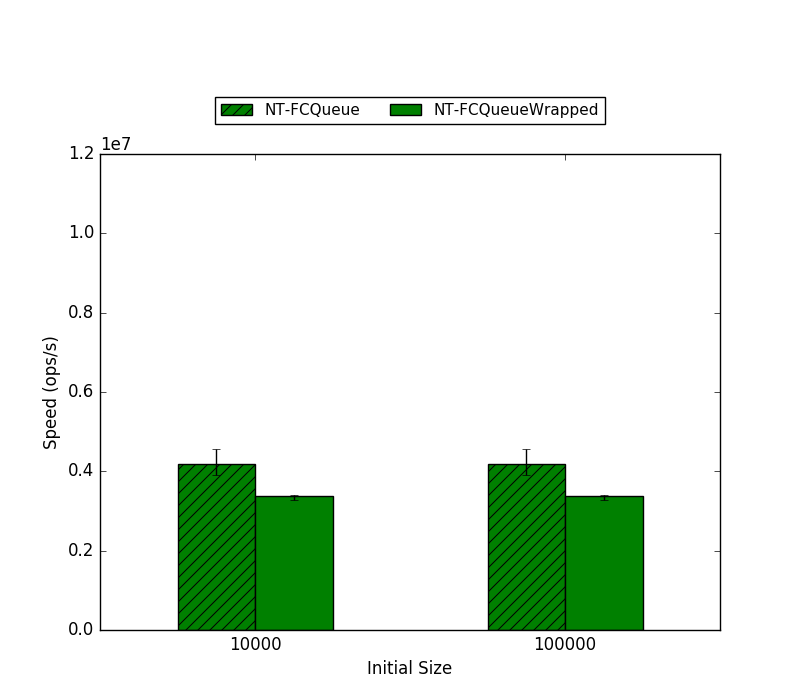
\includegraphics[width=\textwidth]{fcqueues/ntQ:PushPop.png}}
        \caption*{Push-Pop Test (2 threads)}
        \vspace{12pt}
	\end{minipage}
   	\begin{minipage}{0.75\textwidth}
        \boxed{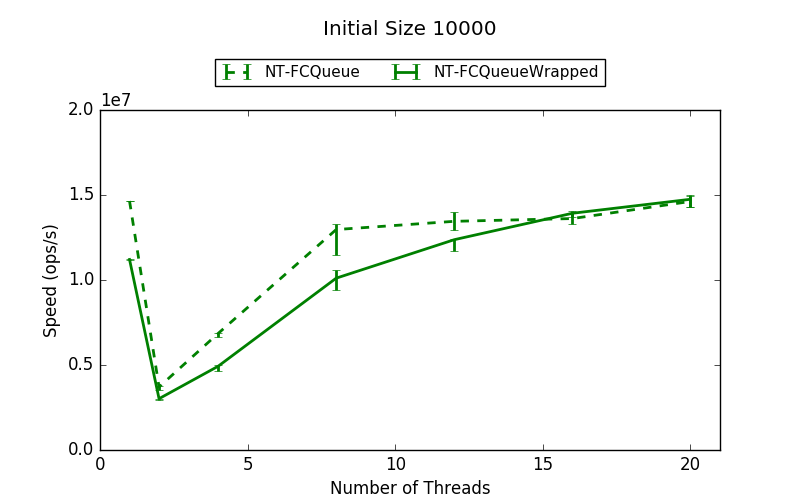
\includegraphics[width=\textwidth]{fcqueues/ntQ:RandSingleOps10000.png}}
        \caption*{Multi-Thread Singletons Test}
	\end{minipage}
        \caption{NT-FCQueue vs. NT-FCQueueWrapped Performance}
    \label{fig:wrappedqs}
\end{figure}

We create a version of the NT-FCQueue, called NT-FCQueueWrapped, that invokes general STO bookkeeping calls. The relative performance of the NT-FCQueueWrapped to the NT-FCQueue indicates how much of the overhead added by the STO system is unavoidable (without modifying STO itself). 
Selected results are shown in Figure~\ref{fig:wrappedqs}.

\begin{figure}[H]
\centering
\singlespace
\lstset{
	language=C++,
	basicstyle=\ttfamily\small,
	keywordstyle=\color{blue}\ttfamily,
	stringstyle=\color{red}\ttfamily,
	commentstyle=\color{green}\ttfamily,
	morekeywords={true, false},
}
	\begin{lstlisting}
		Sto::start_transaction();
		try {
			do_queue_op(push, 1);
			do_queue_op(pop, 0);
			if (Sto::try_commit()) {
				printf("committed");
			}
		} catch (Transaction::Abort e) {
			printf("aborted");
		}
	\end{lstlisting}
\caption{Example usage of STO wrapper calls}
\label{fig:wrappers}
\end{figure}

The STO wrapper functions called by NT-FCQueueWrapped must be called by any user of the data structure in order for the data structure to perform the necessary bookkeeping to support transactions.
These two calls are \texttt{start\_transaction} and \texttt{try\_commit}, and allow a user to mark which operations should occur together in the same transaction. An example of how these calls are used are in Figure~\ref{fig:wrappers}. After invoking the \texttt{start\_transaction} call, the thread is able to collect items in its read- and write-sets. At the end of a transaction, the thread invokes the \texttt{try\_commit} call to run the commit protocol. The NT-FCQueueWrapped adds no items to the read- and write-sets after invoking \texttt{start\_transaction} and does nothing in its commit protocol. This means that the NT-FCQueueWrapped incurs the minimum amount of overhead necessary to use STO and therefore represents the upper bound on the performance we can expect from a fully transactional flat combining queue: the T-FCQueue. 

The STO wrapper calls can lead to a loss of performance ranging from 0\% at twenty threads to 40\% at four threads compared to the performance of the vanilla non-transactional flat combining queue. 
 With fewer threads accessing the queue, the proportion of overhead from the STO wrapper calls is greater because the overhead from synchronizing access to the queue is minimal. As the number of threads increases, the STO wrapper call overhead becomes negligible in comparison to the cost of synchronization.
The NT-FCQueueWrapped scales nearly equally as well as the NT-FCQueue, and the performance of the two queues becomes nearly equivalent at 12 threads with initial queue size 10000.


This comparison of the NT-FCQueueWrapped and the NT-FCQueue demonstrates that STO introduces unavoidable overhead that becomes negligible at high thread counts. Even with the wrapper calls, our results indicate it can still be possible to achieve performance up to nearly 2$\times$ greater at 20 threads than that of the T-QueueP.

\vspace{12pt}
\noindent\fbox{\begin{minipage}{\textwidth}
    \textbf{SUPPORTED}: Adding the calls to the general STO wrapper functions that are necessary for any data structure to support transactions does not cripple the performance of highly-concurrent queues such as the NT-FCQueue, particularly at high thread counts.
\end{minipage}}

\subsubsection{Hypothesis 5: A transactional flat combining queue outperforms and scales better than a transactional queue with a naive concurrent algorithm.}
\label{eval:hypo5}

\begin{figure}[H]
    \centering
	\begin{minipage}{0.75\textwidth}
        \boxed{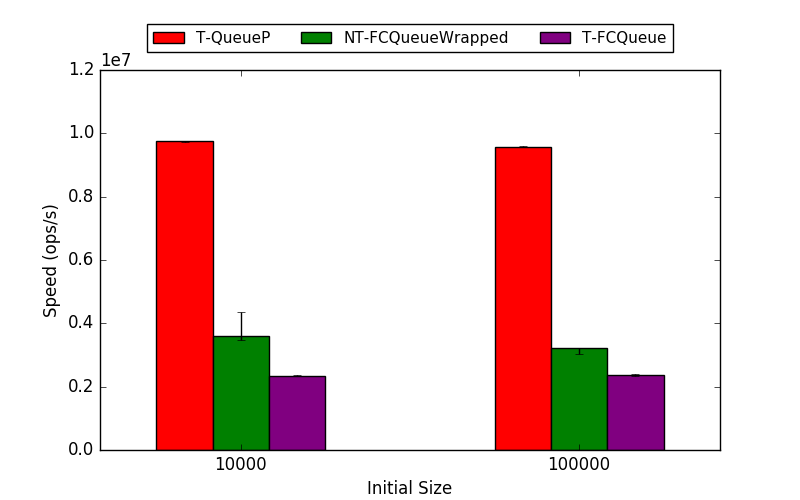
\includegraphics[width=\textwidth]{fcqueues/tQ:PushPop.png}}
        \caption*{Push-Pop Test}
        \vspace{12pt}
	\end{minipage}
   	\begin{minipage}{0.75\textwidth}
        \boxed{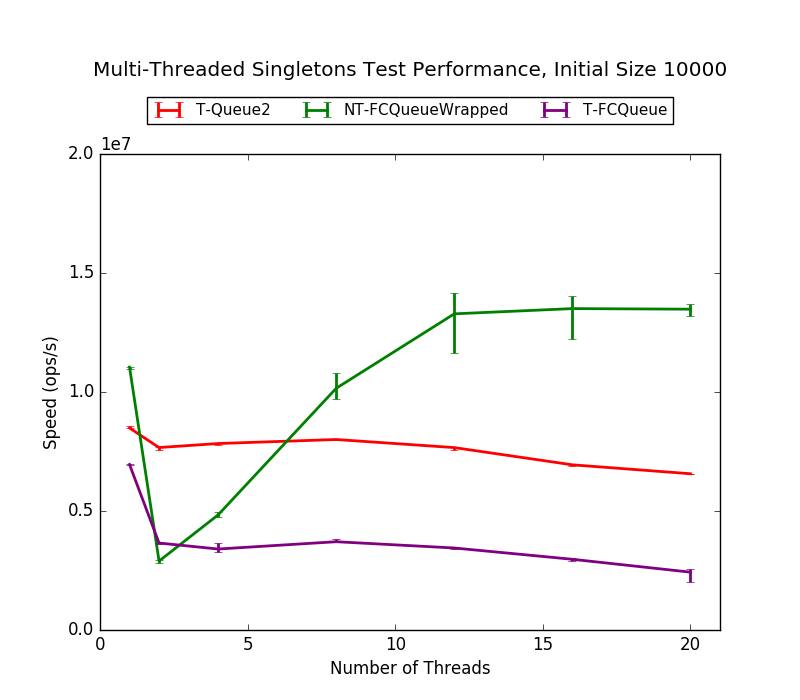
\includegraphics[width=\textwidth]{fcqueues/tQ:RandSingleOps10000.png}}
        \caption*{Multi-Thread Singletons Test}
	\end{minipage}
        \caption{T-FCQueue Performance}
    \label{fig:tqs}
\end{figure}

We compare the T-FCQueue against the NT-FCQueueWrapped and the T-QueueP to measure how the flat combining transactional approach described in Section~\ref{fcqueuet} performs. Selected results are shown in Figure~\ref{fig:tqs}.

In the Push-Pop Test (Figure~\ref{fig:tqs}), the T-QueueP outperforms both flat combining variants. This is an unsurprising result given our results from the concurrent queues benchmark in Figure~\ref{fig:ntqs}. We also note that only the T-QueueP experiences aborts (at approximately a 1.2\% abort rate). We hypothesize that this is due to a potential ``starvation'' property of the T-QueueP: the T-QueueP's pop or push operations acquire a global queue lock, which means that the push-only or pop-only thread may continuously succeed in acquiring the lock. This would lead to a large sequence of pops or pushes, and therefore a greater likelihood that the queue reaches an empty state; this is the only state that can cause the transaction to abort, other than reaching the spin bound when attempting the acquire the queue lock.
The flat combining algorithm, however, applies the operations of both requesting threads during one combiner pass. Since one thread only pushes and the other only pops, no thread aborts due to seeing a marked pop, and the queue rarely reaches an empty state (both one push and one pop are applied during each pass). While not particularly important for performance, flat combining does offer a nice ``no-starvation'' property in this particular situation.

The Multi-Threaded Singletons Test (Figure~\ref{fig:tqs}) shows that the T-QueueP performs approximately 2$\times$ better than the T-FCQueue, regardless of initial queue size. Both queues do not scale, and the performance ratio remains constant regardless of the number of threads. The T-FCQueue also experiences abort rates $1.5$--$2\times$ of that of the T-QueueP.

\vspace{12pt}
\noindent\fbox{\begin{minipage}{\textwidth}
\textbf{NOT SUPPORTED}: The transactional flat combining queue does not outperform and scale better than our other transactional queues. The T-FCQueue's poor performance compared to that of the T-QueueP demonstrates that the flat combining algorithm performs poorly when modified to support transactions.
\end{minipage}}

\subsubsection{Conclusion}
Analysis with the \texttt{perf} tool indicates that the majority of the T-FCQueue's overhead comes from spinning on the flat combining lock (acquired by the combiner thread) or waiting for a flat combining call to complete. In addition, the number of cache misses is over 4$\times$ greater than that of the NT-FCQueue (see Figure~\ref{fig:qcm}). This overhead occurs for two reasons:
\begin{enumerate}
    \item \emph{Higher Quantity}: As described in Section~\ref{fcqueuet}, a thread must make multiple flat combining calls to perform a pop within a transaction (recall that a push only requires one flat combining call).
\item \emph{Higher Complexity}: each flat combining call requires executing instructions, which makes each operation request more expensive.
\end{enumerate}

We conclude that the flat combining technique, while perhaps near-optimal for a highly-concurrent data structure, is no better in a transactional setting than a naive synchronization technique such as that used in the T-QueueO and T-QueueP. The flat combining algorithm must track the state of the queue during the transaction's lifetime to provide transactional guarantees (e.g., marking values in the queue or observing that the queue was empty when performing a pop). This requires modifying the flat combining algorithm itself, which reduces the performance benefits derived from the algorithm's optimizations. In the next chapter, we formalize this argument using a commutativity discussion and claim that the higher quantity of more complex flat combining calls is necessary for flat combining to be used in a transactional setting: the flat combining technique depends on operation commutativity present in only a non-transactional setting to achieve its high performance. 

\iffalse
For ease of reference, we list here the names of queues discussed in this section. Their meaning is explained in context with more detail within the discussion.
\begin{itemize}
    \item T-QueueO: the optimistic, transactional, and naively-concurrent queue.
    \item T-QueueP: the transactional and naively-concurrent queue that performs pessimistic locking upon performing a pop.
    \item NT-FCQueue: the non-transactional flat combining queue.
    \item NT-FCQueueWrapped: a version of NT-FCQueue that invokes STO \texttt{start\_transaction} and \texttt{commit\_transaction} calls.
    \item T-FCQueue: the fully-transactional flat-combining queue.
\end{itemize}

\fi
